% Animated SAFAID inference pipeline: one frame per (\stage, \variant).
% Build all frames and the GIF with:  bash assets/src/make_animation.sh
%   \stage   1 input | 2 prompt | 3 vision encoder | 4 merger | 5 LLM decoder | 6 response
%   \variant 0 answer "real" | 1 answer "AI-generated"
\documentclass[tikz,border=0pt]{standalone}
\usepackage[T1]{fontenc}
\usepackage{helvet}
\renewcommand{\familydefault}{\sfdefault}
\usetikzlibrary{positioning,arrows.meta,calc}
\providecommand{\stage}{6}
\providecommand{\variant}{0}

\definecolor{paper}{HTML}{FCFCFB}
\definecolor{inGrey}{HTML}{F2F2F2}   \definecolor{inEdge}{HTML}{8C8C8C}
\definecolor{prBlue}{HTML}{E3F0FB}   \definecolor{prEdge}{HTML}{2A78D6}
\definecolor{mdYell}{HTML}{FFF4D6}   \definecolor{mdEdge}{HTML}{E0A100}
\definecolor{subFill}{HTML}{FFE8A3}  \definecolor{subHot}{HTML}{FFC83D}
\definecolor{okFill}{HTML}{E4F4E4}   \definecolor{okEdge}{HTML}{2E8B3E}
\definecolor{bdFill}{HTML}{FCE6E6}   \definecolor{bdEdge}{HTML}{C8413F}
\definecolor{ink}{HTML}{1F1F1F}      \definecolor{muted}{HTML}{5A5A5A}

\begin{document}
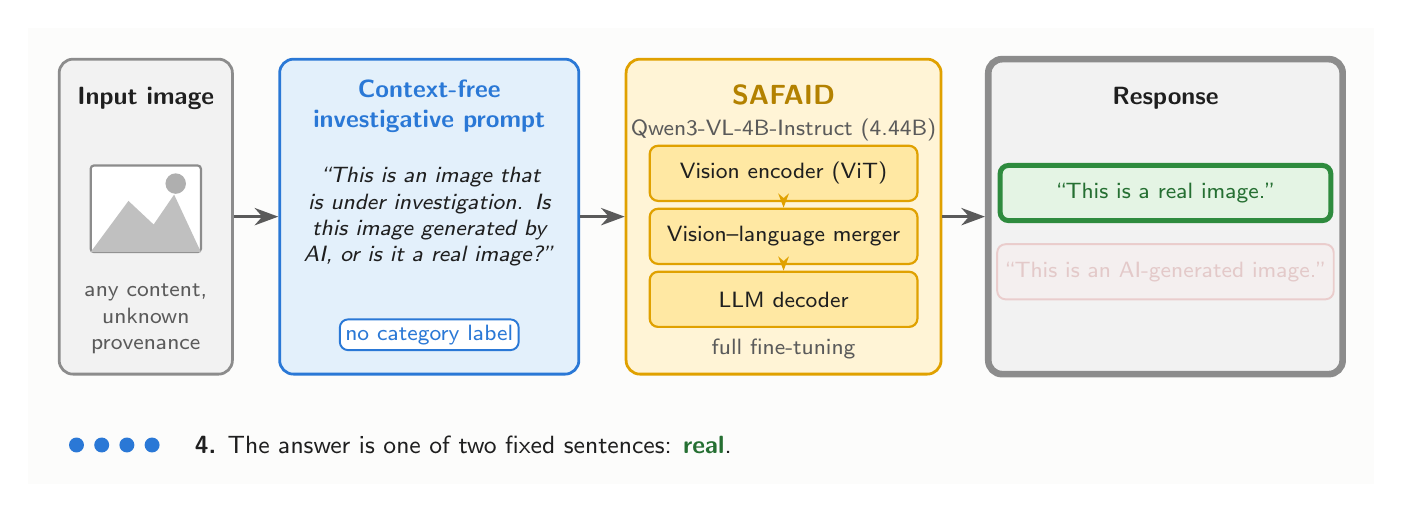
\begin{tikzpicture}[x=1mm, y=1mm, font=\small, text=ink,
    box/.style={rounded corners=5pt, align=center},
    sub/.style={rounded corners=3pt, minimum width=34mm, minimum height=7mm, align=center, font=\footnotesize},
    tag/.style={rounded corners=3pt, inner sep=2pt, font=\footnotesize},
    flow/.style={-{Stealth[length=3mm,width=2.2mm]}, line width=1.1pt, draw=muted}]
  % opacity of each block (reached or not) and border width (active or not)
  \pgfmathsetmacro{\oPr}{ifthenelse(\stage>=2,1,0.22)}
  \pgfmathsetmacro{\oMd}{ifthenelse(\stage>=3,1,0.22)}
  \pgfmathsetmacro{\oOut}{ifthenelse(\stage>=6,1,0.22)}
  \pgfmathsetmacro{\wIn}{ifthenelse(\stage==1,2.4,1)}
  \pgfmathsetmacro{\wPr}{ifthenelse(\stage==2,2.4,1)}
  \pgfmathsetmacro{\wMd}{ifthenelse(and(\stage>=3,\stage<=5),2.4,1)}
  \pgfmathsetmacro{\wOut}{ifthenelse(\stage==6,2.4,1)}
  \pgfmathsetmacro{\oReal}{ifthenelse(\variant==0,1,0.2)}
  \pgfmathsetmacro{\oFake}{ifthenelse(\variant==1,1,0.2)}

  % canvas (fixed size for every frame)
  \fill[paper] (-4,-34) rectangle (167,24);

  % ---------------- input image
  \node[box, draw=inEdge, fill=inGrey, line width=\wIn pt, minimum width=22mm, minimum height=40mm] (img) at (11,0) {};
  \node[font=\small\bfseries] at (11,15) {Input image};
  \begin{scope}[shift={(11,1)}]
    \draw[inEdge, line width=0.8pt, rounded corners=1.2pt, fill=white] (-7,-5.5) rectangle (7,5.5);
    \ifnum\variant=0
      \fill[inEdge!55] (-7,-5.5) -- (-2.2,1) -- (1,-2) -- (3.6,1.8) -- (7,-5.5) -- cycle;
      \fill[inEdge!70] (3.8,3.2) circle (1.3);
    \else
      \fill[inEdge!70] (0,1.7) circle (2.1);
      \begin{scope}
        \clip[rounded corners=1.2pt] (-7,-5.5) rectangle (7,5.5);
        \fill[inEdge!55] (-5.4,-5.5) .. controls (-5.2,-0.9) and (5.2,-0.9) .. (5.4,-5.5) -- cycle;
      \end{scope}
    \fi
  \end{scope}
  \node[font=\footnotesize, text=muted, align=center] at (11,-13) {any content,\\unknown\\provenance};

  % ---------------- prompt
  \begin{scope}[opacity=\oPr]
    \node[box, draw=prEdge, fill=prBlue, line width=\wPr pt, minimum width=38mm, minimum height=40mm] (pr) at (47,0) {};
    \node[font=\small\bfseries, text=prEdge, align=center] at (47,14) {Context-free\\investigative prompt};
    \node[font=\footnotesize\itshape, align=center, text width=34mm] at (47,0)
         {``This is an image that is under investigation. Is this image generated by AI, or is it a real image?''};
    \node[tag, draw=prEdge, fill=white, text=prEdge, line width=0.7pt] at (47,-15) {no category label};
  \end{scope}

  % ---------------- SAFAID model
  \begin{scope}[opacity=\oMd]
    \node[box, draw=mdEdge, fill=mdYell, line width=\wMd pt, minimum width=40mm, minimum height=40mm] (md) at (92,0) {};
    \node[font=\normalsize\bfseries, text=mdEdge!80!black] at (92,15.5) {SAFAID};
    \node[font=\footnotesize, text=muted] at (92,11) {Qwen3-VL-4B-Instruct (4.44B)};
    \foreach \name/\y/\k/\lab in {ve/5.5/3/{Vision encoder (ViT)}, mg/-2.5/4/{Vision--language merger}, lm/-10.5/5/{LLM decoder}} {
      \pgfmathsetmacro{\hot}{ifthenelse(\stage==\k,1,0)}
      \ifdim\hot pt>0pt
        \node[sub, draw=mdEdge!70!black, fill=subHot, line width=1.6pt] (\name) at (92,\y) {\textbf{\lab}};
      \else
        \node[sub, draw=mdEdge, fill=subFill, line width=0.8pt] (\name) at (92,\y) {\lab};
      \fi
    }
    \draw[-{Stealth[length=1.8mm]}, line width=0.7pt, draw=mdEdge] (ve) -- (mg);
    \draw[-{Stealth[length=1.8mm]}, line width=0.7pt, draw=mdEdge] (mg) -- (lm);
    \node[font=\footnotesize, text=muted] at (92,-16.8) {full fine-tuning};
  \end{scope}

  % ---------------- response
  \begin{scope}[opacity=\oOut]
    \node[box, draw=inEdge, fill=inGrey, line width=\wOut pt, minimum width=45mm, minimum height=40mm] (out) at (140.5,0) {};
    \node[font=\small\bfseries] at (140.5,15) {Response};
  \end{scope}
  % both answers stay equally dim until the response stage
  \pgfmathsetmacro{\oA}{ifthenelse(\stage>=6,\oReal,0.22)}
  \pgfmathsetmacro{\oB}{ifthenelse(\stage>=6,\oFake,0.22)}
  \pgfmathsetmacro{\wA}{ifthenelse(and(\stage==6,\variant==0),1.8,0.7)}
  \pgfmathsetmacro{\wB}{ifthenelse(and(\stage==6,\variant==1),1.8,0.7)}
  \node[tag, opacity=\oA, draw=okEdge, fill=okFill, text=okEdge!80!black, line width=\wA pt, minimum width=42mm, minimum height=7mm] at (140.5,3)
       {``This is a real image.''};
  \node[tag, opacity=\oB, draw=bdEdge, fill=bdFill, text=bdEdge!80!black, line width=\wB pt, minimum width=42mm, minimum height=7mm] at (140.5,-7)
       {``This is an AI-generated image.''};

  % ---------------- flow arrows (visible once their target is reached)
  \draw[flow, opacity=\oPr] (img.east) -- (pr.west);
  \draw[flow, opacity=\oMd] (pr.east) -- (md.west);
  \draw[flow, opacity=\oOut] (md.east) -- (out.west);

  % ---------------- caption strip: step dots and one line of text
  \foreach \i in {1,...,4} {
    \pgfmathsetmacro{\cur}{ifthenelse(\stage==1,1,ifthenelse(\stage==2,2,ifthenelse(\stage==6,4,3)))}
    \pgfmathsetmacro{\isOn}{ifthenelse(\i<=\cur,1,0)}
    \ifdim\isOn pt>0pt \fill[prEdge] (-1+\i*3.2,-29) circle (0.95); \else \draw[muted, line width=0.6pt] (-1+\i*3.2,-29) circle (0.95); \fi
  }
  \node[anchor=west, font=\small, text=ink] at (16,-29) {%
    \ifcase\stage\or
      \textbf{1.} Any image: no category label, unknown provenance.\or
      \textbf{2.} The same forensic question for every image, in training and at test time.\or
      \textbf{3.} One fully fine-tuned vision--language model reads the image and the question.\or
      \textbf{3.} One fully fine-tuned vision--language model reads the image and the question.\or
      \textbf{3.} One fully fine-tuned vision--language model reads the image and the question.\or
      \ifnum\variant=0 \textbf{4.} The answer is one of two fixed sentences: \textcolor{okEdge!80!black}{\textbf{real}}.\else
                       \textbf{4.} The answer is one of two fixed sentences: \textcolor{bdEdge!80!black}{\textbf{AI-generated}}.\fi
    \fi};
\end{tikzpicture}
\end{document}
